\chapter{Background}

In this chapter we will go through the fundamental mathematics and concepts behind the \textit{Convolutional Neural Network} (CNN) model. It gives a basic introduction to both general neural networks and \textit{CNNs}.

\section{Artificial Neural Networks}\label{ann}

An \textit{Artificial Neural Network} (ANN) \cite{Minsky1969}\cite{Bishop2006} is a computational model that is used for machine learning and pattern recognition. The name and basic concept is inspired by how the animal brain uses a network of neurons to recognize and classify objects. Depending on the input different neurons \textit{activate} (or \textit{fire}), making the brain able to decide what kind of pattern it is detecting. 

An ANN can intuitively be viewed as a probabilistic classifier. Depending on the input data it will calculate the probability that the data belongs to a certain \textit{class} (e.g. an object in an image or an investment decision). The network can be trained to recognize different classes by being provided a set of labeled training data, e.g. a set of faces and a set of non-faces. It can then learn to decide whether a image contains a face or not. This is called supervised learning. The network can also be trained unsupervised, by providing it with a set of unlabeled images. It will then learn to recognize a set of classes, but will be unable to label them.  

\subsection{Definition} \hfill \break
An ANN  consists of a number of layers containing a set of so-called \textit{neurons}, also known as \textit{units}. A neuron takes in a set of values as input (e.g. image pixels), where each value is associated with a respective weight. The input and the weights are multiplied and summed, and the result is used to calculate a non-linear \textit{activation function}. Formally a neurons input and output is defined as:


\begin{equation}\label{eq_neuron_in}
Input: \{x_1, x_2,\dots, x_n\} = \mathbf{x} 
\end{equation}

\begin{equation}\label{eq_neuron_out}
Output: f(\mathbf{w^{T}x)} = f(\sum_{i=1}^{n}w_i x_i + b) = o
\end{equation}

Where \textbf{w} is the connection weights and b is the neuron bias. \textit{f(...)} is the activation function, which eumulates the activation of a neuron in the brain. It also causes the values in the network to have a reasonable value interval. \textit{f(...)} tends to be either:

\begin{equation}
Sigmoid: f(z) = \frac{1}{1 - e^{-z}}
\end{equation}



\begin{equation}
\text{Hyperbolic tagent:} f(z) = tanh(z) = \frac{e^z - e^{-z}}{e^z + e^{-z}}
\end{equation}



Figure \ref{fig_neuron} provides a visualization of the functionality of a neuron. 

\begin{figure}[h!]
  \centering
      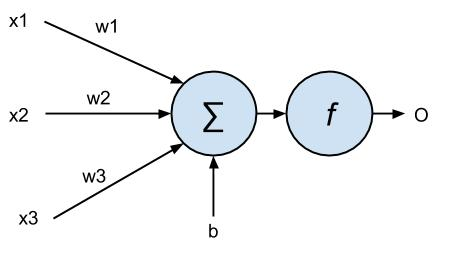
\includegraphics[width=0.5\textwidth, scale=0.1]{Figures/Background/Neuron}
  \caption{A single neuron with three inputs. }
  \label{fig_neuron}
\end{figure}

An ANN consist of $ n_l $ layers, each containing a set of neurons. The first layer is \textit{the input layer}, and the last layer is \textit{the output layer}. The layers in between are called \textit{the hidden layers}. Each layer uses the previous layer's output as input. The input layer is provided with the initial input and uses it to calculate the activation function for each of its neurons. The result is propagated to the first hidden layer, and continues up until it reaches the output layer, which provides the final output. This is known as a \textit{feedforward neural network.}

The network takes in two parameters, $ (\mathbf{W, b}) = (\mathbf{w}^{(1)}, b^{(1)}, 
\mathbf{w}^{(2)}, b^{(2)}, \dots , 
\mathbf{w}^{(n_l)}, b^{(n_l)}) $. $ w_{ij}^l $ denotes the weight between neuron j in layer l, and neuron i in layer l+1. $ b_i^l $ denotes the bias associated with the neurons in layer l+1. Note that upper case bold is a matrix, lower case bold is a vector, and lower case not bold is a scalar. 


\begin{figure}[h!]
  \centering
      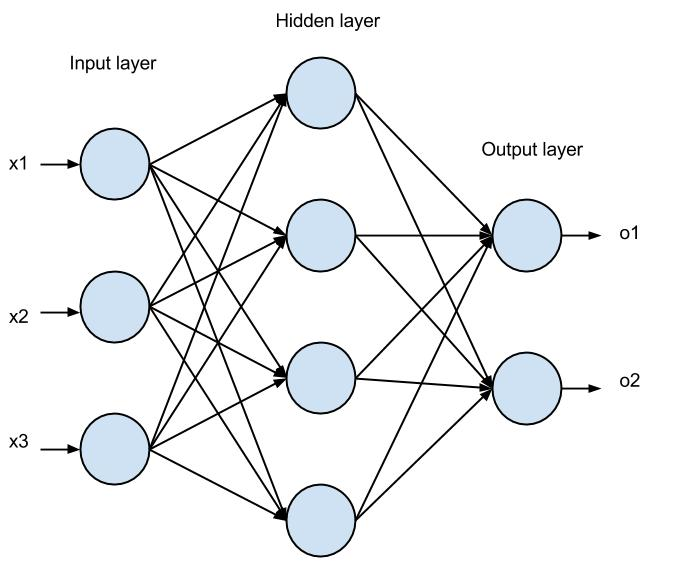
\includegraphics[width=0.5\textwidth]{Figures/Background/ann}
  \caption{An Artificial Neural Network.}
\end{figure}


\subsection{Training} \label{sec_ann_training}
During the training of the network it is the parameters $ (\mathbf{W, b}) $ that are altered in order to adapt the network to the training data. This is done by providing the network with a set of training samples, where we provide an input and an expected output. By using a cost function we can then figure out how we should tune our weights and biases in order to reduce the error rate. In other words, our goal is to minimize a cost function over a set of training samples. This can be done by using \textit{gradient decent} and the \textit{backpropagation algorithm} \cite{Rumelhart1986}\cite{Leonard1990}\cite{LeCun1998}. 

Let the cost function for a single training example $(x,y)$ be defined as:

\begin{equation}
	Cost(\mathbf{W},\mathbf{b}; x, y) = \frac{1}{2}(h_{\mathbf{W},\mathbf{b}}(x) - y)^2
\end{equation}

Where $ x $ is the input, $ h_{\mathbf{w},b}(x) $ is the actual output of our network and \textit{y} is the correct output.
Then the cost function for \textit{m} training examples $ ((x^{1}, y^{1}), (x^{2}, y^{2}), \dots, (x^{m}, y^{m})) $ is:

\begin{equation}
	Cost(\mathbf{W},\mathbf{b}) = \frac{1}{m}\sum_{i=1}^{m}Cost(\mathbf{W},\mathbf{b};x^{(i)},y^{(i)}) + \frac{\lambda}{2}
	\sum_{l=1}^{n_l-1}\sum_{i=1}^{s_l}\sum_{j=1}^{s_l+1}
	(\mathbf{w}_{ji}^{l})^2
\end{equation}
 
Where the first term is simply the average sum-of-squares error. The second term is the \textit{regularization term}, or \textit{weight decay term}, which tends to reduce \textit{overfitting}. ANNs have a vast number of parameters, i.e. weights, and makes it susceptible to random noise. This can greatly reduce the networks ability to provide correct predictions, But this  can be mended by the regularization term. 

Based on this we can use gradient decent to compute how we should alter the weights in order to reduce the cost function. One iteration of gradient descent updates \textbf{w} and \textit{b} as follows:

\begin{equation}
	w_{ij}^{(l)} = w_{ij}^{(l)} - \alpha\frac{\partial}{\partial w_{ij}^{(l)} }Cost(\mathbf{W},\mathbf{b})
\end{equation}

\begin{equation}
	b^{(l)} = b^{(l)} - \alpha\frac{\partial}{\partial b_{i}^{(l)} }Cost(\mathbf{W},\mathbf{b})
\end{equation}

Where $ \alpha $ is the learning rate, which is a predetermined constant. Note that this would only make us able to compute the gradient for the output layer. In order to perform gradient decent on the hidden layers, we need to propagate the error from the output layer backwards, to the hidden layers. For this we use the \textit{backpropagation algorithm}. Let $ o_i^{(l)} $ denote the output of the $i$th neuron in layer $l$, and $z_k^{(l)}$ is the weighted sum of the inputs plus the bias for the $k$th neuron in layer l. Then the \textit{backpropagation algorithm} can be formalized as follows: 

\begin{enumerate}
	\item Perform a feedforward pass, computing the output of every layer.
	\item For each output neuron k in the output layer, compute \textit{the error term}: 
	\begin{equation}
		\delta_k = \frac{\partial}{\partial z_{k}^{(n_l)} }Cost(\mathbf{W,b}; x, y) = -o_k^{n_l}(1-o_k^{n_l})(y_k-o_k^{n_l})
	\end{equation} 
	\item For each hidden layer $ l = n_l - 1, n_l - 2,\dots, 2 $ compute: 
	\begin{equation}
		\delta_i^{l} = o_i^l(1-o_i^l)\sum_{j=1}^{s_{l+1}} w_{ij}^l \delta_j^{l+1} 
	\end{equation}
	\item Compute the partial derivative for each weight and bias:
	\begin{equation}
		\frac{\partial}{\partial w_{ij}^{(l)} }Cost(\mathbf{W,b}; x, y) = o_j^{(l)}\delta_i^{(l+1)}
	\end{equation}
	
	\begin{equation}
		\frac{\partial}{\partial b^{(l)} }Cost(\mathbf{W,b}; x, y) = \delta_i^{(l+1)}
	\end{equation}
\end{enumerate}
	
Now, combining \textit{gradient decent} and the \textit{backpropagation algorithm} we can describe an algorithm to train our network: 

\begin{enumerate}
	\item Initialize the weights $ \mathbf{w}^{(l)} $ and $ b^{l} $ to random values for every layer \textit{l}.
	\item Do steps 3 to 5 until the $ Cost(\mathbf{W, b}) $ function is low enough or converges. This is referred to as an \textit{epoch}. 
	\item Set $ \Delta\mathbf{w}^{(l)} := 0 $ and $ \Delta b^{(l)} := 0 $ for all \textit{l}.
	\item For i = 1 to m,
		\begin{enumerate}
			\item Use the backpropagation algorithm to compute $ \nabla_\mathbf{w^{(l)}}Cost(\mathbf{W, b};x^{(i)},y^{(i)}) $ and $ \nabla_b^{(l)}Cost(\mathbf{W, b};x^{(i)},y^{(i)}) $ for every layer \textit{l}.
			\item  Set $ \Delta\mathbf{w}^{(l)} := \Delta\mathbf{w}^{(l)} + \nabla_\mathbf{w^{(l)}}Cost(\mathbf{W, b};x^{(i)},y^{(i)}) $. 
			\item  Set $ \Delta b^{(l)} := \Delta b^{(l)} + \nabla_{b^{(l)}}Cost(\mathbf{W, b};x^{(i)},y^{(i)}) $. 
		\end{enumerate}
	\item Update the parameters:
		\begin{equation*}
			\mathbf{w}^{(l)} = \mathbf{w}^{(l)} - \alpha[(\frac{1}{m}\Delta\mathbf{w}^{(l)}) + \lambda\mathbf{w}^{(l)}]
		\end{equation*}
		
		\begin{equation*}
			b^{(l)} = b^{(l)} - \alpha[\frac{1}{m}\Delta b^{(l)}]
		\end{equation*}
\end{enumerate}

\subsection{Issues with object recognition}\label{ann_issues}

The standard ANN model face three issues when it comes to object recognition in images \cite{LeCun1998}. 

\begin{enumerate}

	\item A fully connected ANN does not take into consideration the topology of the input. An image has a strong 2D spatial locality correlation, which makes it possible to combine low-order features (edges, end-points etc.) in the same area into higher-order features.  
	
	\item Even small images contains a large amount of pixels/inputs, e.g. a $ 32 \times 32 $ image contains 1024 pixels/inputs. A fully connected network with 100 hidden units would then end up with $ 1024 \times 100 $ weights that needs to be calculated in the first layer, making harder to scale for larger images and inefficient .
	
	\item While objects are similar enough on a higher level to be grouped together into a class, they can still be very different on a lower level. E.g. a human face have several features that are needed for it to be defined as a face, e.g. eyes, mouth, nose etc. But the size and shape of these features tend to be very different from person to person. While it is possible for a standard ANN to compensate for these internal differences within a class, the network would have to be very large, would probably contain several neurons with similar weight vectors positioned at different places in the network, and would require a very large number of training samples. 
	
\end{enumerate}



% % % % % % % % % % % % % % % % % % % % % % % % % % % % % % % % % % % %
%CONVNET!
% % % % % % % % % % % % % % % % % % % % % % % % % % % % % % % % % % % % 
\section{Convolutional Neural Network}\label{cnn}

A \textit{Convolutional Neural Network} \cite{LeCun1998} (CNN) is an extension of the \textit{Artificial Neural Network} model, which is made specificly for object recognition in images or speech recognition. It was made in order to solve the issues that the classic ANN model faced 


\begin{figure}[h!]
  \centering
      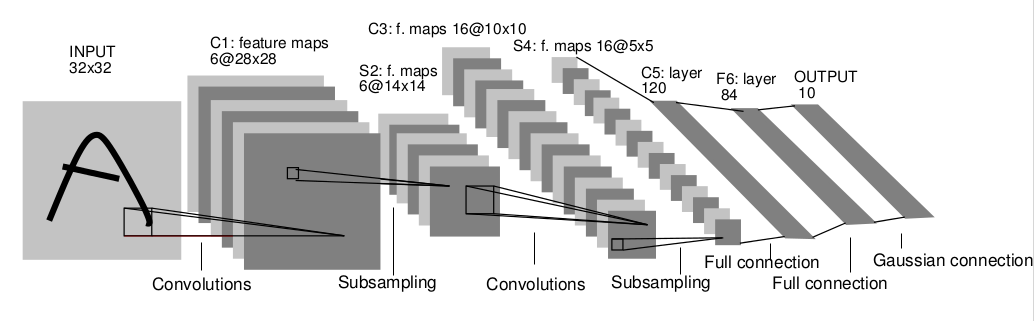
\includegraphics[width=1.0\textwidth]{Figures/Background/convnet}
  \caption{An example CNN, the LeNet-5 \cite{LeCun1998}. }
  \label{fig_cnn}
\end{figure}

\subsection{Definition} \hfill \break

The CNN model adds two additional types of layers, in addition to the standard ANN layers: a \text{convolution layer} and a \textit{subsampling/pooling layer}. The idea behind the two new layers is to exploit the strong 2D local structure of images, i.e. pixels close to each other are highly correlated. By using local correlation one can extract and combine small local features (e.g. edges, corners, points) into higher-order features (e.g. nose, mouths, forehead), which can in the end be recognized as an object (e.g. a face).  A full network is illustrated in Figure \ref{fig_cnn}


\paragraph{Convolution layer}  \hfill \break
Intuitively, the convolution layer performs the feature extraction by applying a filter (kernel) on the whole image, and puts the result in a corresponding feature map. E.g. if the filter extracts vertical edges, only the vertical edges from the original image would remain in the resulting feature map. Thus different features can be extracted by having several feature maps with different filters.  

Formally we can define a 2D convolution as:

\begin{equation}
\mathbf{F} = \mathbf{X*W}
\end{equation}

Where \textbf{F} is the feature map matrix, X is the input matrix and \textbf{W} is the kernel matrix. Then the actual calculation can be defined as:

\begin{equation}
f_{ij} = \sum_{m=1}^{k}\sum_{n=1}^{k} x_{i+m, j+n}w_{mn}
\end{equation}

Where $ x_{ij} $ is a value of the input matrix, $ w_{mn} $ is a value in the $ k \times k $ kernel matrix, and $ f_{ij} $ is a value of the feature map matrix. Figure \ref{fig_conv_ss_mp} illustrates this operation.

This helps solve the first two issues from Section \ref{ann_issues}. The neurons in a feature map share the same kernel, thus the same weights, which greatly reduces the size of the network. The convolution operation applies a 2D filter on the image, which makes the network able to exploit the spatial correlation in the image. 

\paragraph{Subsampling/pooling layer}  \hfill \break
Once a feature have been detected, the exact position become less important. For example, the distance between the mouth and the eyes tend to vary between persons. So in order to make the CNN not too sensitive to the relative placement of features, the accuracy of the feature map needs to be reduced. This can be done by subsampling (i.e. partitioning) the feature map into $ s \times s $ non-overlapping matrices, and then perform a pooling operation on each respective matrix. There are two types of pooling operations which are used for CNNs: 

\begin{itemize}
	\item \textit{Max-pooling} extracts the maximum value of the matrix.
	\item \textit{Average-pooling} extracts the average value of all the elements in the matrix.
\end{itemize}

\begin{figure}[h!]
  \centering
      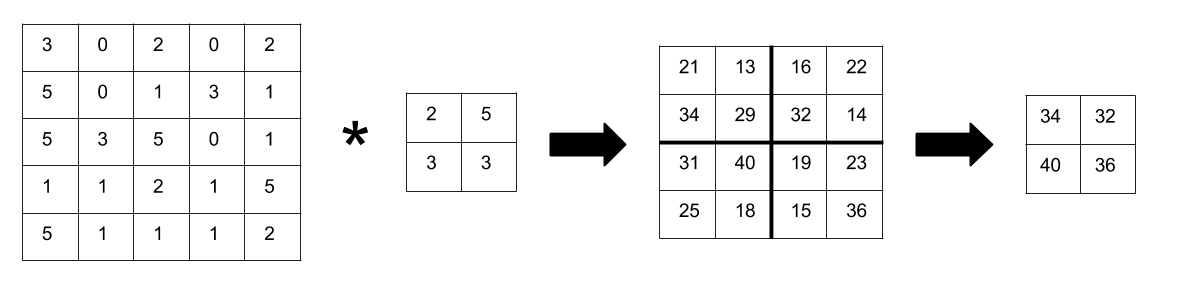
\includegraphics[width=1.0\textwidth]{Figures/Background/Convolution-Maxpooling}
  \caption{Illustration of the convolution and subsampling/max-pooling operations. The leftmost matrix is convulted with a $ 2 \times 2 $ matrix, and the resulting matrix is subsampled into four non-overlapping areas where the max value is extracted.}
  \label{fig_conv_ss_mp}
\end{figure}

\hfill \break

We can then formally define subsampling/pooling as:

\begin{equation}
	\mathbf{O} = subsample\_pool(\mathbf{F})
\end{equation}


Where \textbf{O} is the output matrix, \textbf{F} is the input feature map, and the \textit{subsample\_pool()} function's operation is defined as either:

\begin{equation}
o_{ij} = max(x_{i \times s+p, j \times s+q}) \qquad\qquad q,p \in 1, 2, \dots, s
\end{equation}

or

\begin{equation}
o_{ij} = \frac{1}{s^2} \sum_{p=1}^{s}\sum_{q=1}^{s} x_{i+p, j+q}
\end{equation}

Where $ o_{ij} $ is a value in the output matrix and $ f_{ij} $ is a value in the feature map, and \textit{s} is the dimension of the subsampling size. A max-pooling operation is illustrated in Figure \ref{fig_conv_ss_mp}.

Thus, the subsample/pooling layer helps solve the two last issues from Section \ref{ann_issues}. By reducing the accuracy, the network is less sensitive to the difference between instances of a class. This also causes the network size to be smaller, since it does not require neurons to recognize the differences. 



\paragraph{Training} \hfill \break
As mentioned, a CNN consists of three types of layers: a convolution layer, a subsampling/pooling layer and fully connected layer. The latter is trained as described in the previous section, using backpropagation and gradient decent. The two other layers uses the same general algorithm, but the error $ \delta^l $ and the gradient of $ Cost(\mathbf{W,b}; x, y) $ is calculated differently. . 

Since the backpropagation aglorithm starts at the last layer and work its way backwards, the error is first calculated for the fully connected layer, then provided to the subsampling/pooling layer, and finally to the convolution layer. Thus we first need to calculate the error for the subsampling/pooling layer, so we can propegate it to the convolution layer. 

The subsampling/pooling layer does not contain any weight, and can therefore not be tuned, so it only needs to propegate the error it receives. Depending on which pooling operation is used, there are two respective methods for this:

For max pooling, the error is simply propegated to the neuron that was chosen as the maximum value, while the rest are set to zero. Wheras for average-pooling we have to distrubute the error evenly between all the responsible neurons. We therefore define the function \textit{upsample(...)}, which performs the correct propegation operation depending on the type of pooler. 

We can now formally define how to calculate the error and the gradient by simply replacing the equations in step 3 and 4 in the backpropagation algorithm with the following equations. For simplicity we assume that convolution and subsampling/pooling is done in a single layer \textit{l}.




\begin{equation}
	\delta_{k}^{l} =  upsample( (\mathbf{W}_{k}^l)^T \mathbf{\delta}_{k}^{l+1})\cdot f'(\mathbf{Z}_k^l)
\end{equation}

Where $  (\mathbf{W}_{k}^l)^T $ is the weight matrix in layer \textit{l}, $  \mathbf{\delta}_{j}^{l+1} $ is the error matrix for layer $ l + 1 $, $ f'(\mathbf{Z}_k^l) $ is the matrix containing the derivative of the activation function, and k indexes the filter number. I.e. it contains $ o_{kij}^l(1-o_{kij}^l) $ for every neuron at index \textit{ij} in feature map \textit{k} in layer \textit{l}. 

Using this we can calculate the gradient:

\begin{equation}
	\frac{\partial}{\partial \mathbf{w}_k^{(l)} }Cost(\mathbf{W,b}; x, y) = \sum_{i=1}^{m}(\mathbf{o}_i^{(l)})*\delta_k^{(l+1)}
\end{equation}

\begin{equation}
	\frac{\partial}{\partial b_k^{(l)} }Cost(\mathbf{W,b}; x, y) = \sum\delta_k^{(l+1)}
\end{equation}












